\section*{Введение}

We propose TalkNet, a convolutional non-autoregressive neural model for speech syn\-thesis. The model consists of two feed-forward convolutional networks. The first network predicts grapheme durations. An input text is expanded by repeating each symbol accor\-ding to the predicted duration. The second network generates a mel-spectrogram from the expanded text.

To train a grapheme duration predictor, we add the grapheme duration to the training dataset using a pre-trained Connectionist Temporal Classification (CTC)-based speech recognition model. The explicit duration prediction eliminates word skipping and repeating. Experiments on the LJSpeech dataset show that the speech quality nearly matches auto-regressive models. The model is very compact -- it has 10.8M parameters, almost 3x less than the present state-of-the-art text-to-speech models.

The non-autoregressive architecture allows for fast training and inference.

\begin{figure}[!ht]
\centering
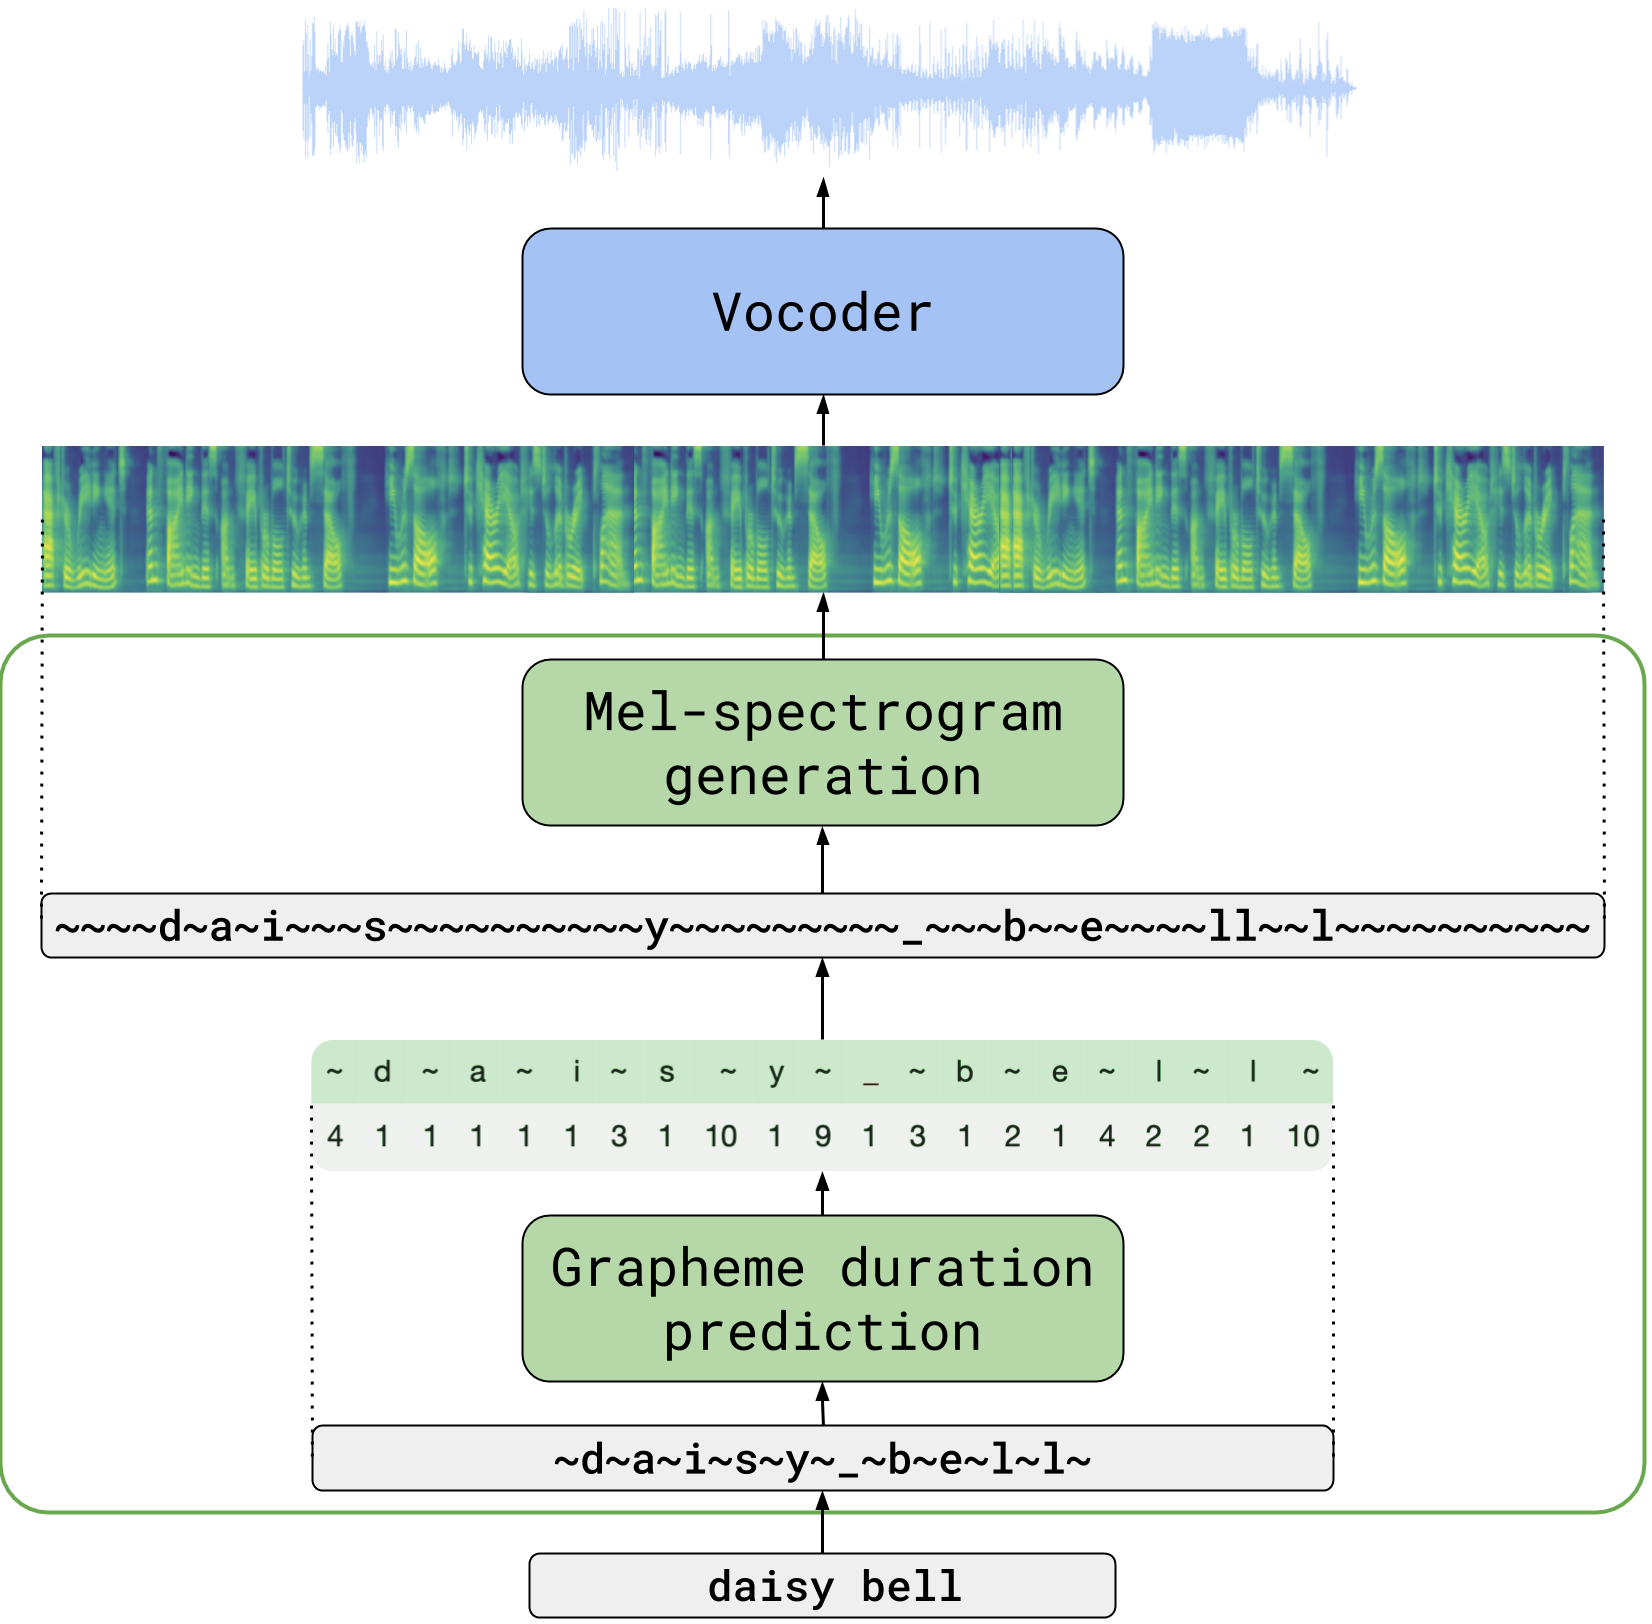
\includegraphics[width=1.0\textwidth]{images/arch.png}
\caption{TalkNet converts text to speech, using a grapheme duration predictor, a mel-spectrogram generator, and a vocoder. We use $\sim$ to denote the CTC blank symbol.}
\label{fig:arch}
\end{figure}